\documentclass{standalone}
\usepackage{graphicx}	
\usepackage{amssymb, amsmath, amsthm}
\usepackage{color}

\usepackage{tikz}
\usetikzlibrary{intersections, backgrounds, math}

\definecolor{light}{RGB}{220, 188, 188}
\definecolor{mid}{RGB}{185, 124, 124}
\definecolor{dark}{RGB}{143, 39, 39}
\definecolor{highlight}{RGB}{180, 31, 180}
\definecolor{gray10}{gray}{0.1}
\definecolor{gray20}{gray}{0.2}
\definecolor{gray30}{gray}{0.3}
\definecolor{gray40}{gray}{0.4}
\definecolor{gray60}{gray}{0.6}
\definecolor{gray70}{gray}{0.7}
\definecolor{gray80}{gray}{0.8}
\definecolor{gray90}{gray}{0.9}
\definecolor{gray95}{gray}{0.95}

\begin{document}

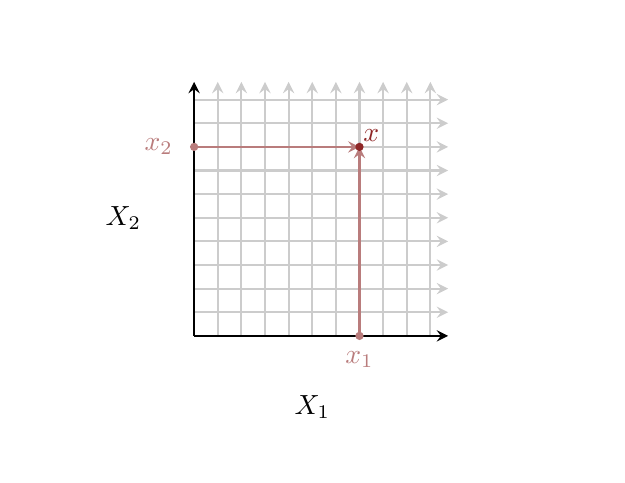
\begin{tikzpicture}[scale=0.30, thick]
  
  \draw[white] (-12, -10) rectangle (12, 8);
  
  \draw[black, line width=0.3, fill=white] (-5, -5) -- (5, -5) -- (5, 5) -- (-5, 5) -- (-5, -5);
  
  \foreach \x in {1, 2, ..., 10} {
    \draw[gray80, ->, >=stealth] (1 * \x - 5, -5) -- (1 * \x - 5, 5.75);
  }

  \foreach \y in {1, 2, ..., 10} {
    \draw[gray80, ->, >=stealth] (-5, 1 * \y - 5) -- (5.75, 1 * \y - 5);
  }
  
  \draw[black, ->, >=stealth] (-5, -5) -- (5.75, -5);
  \node[] at (0, -8) {$X_{1}$};

  \draw[black, ->, >=stealth] (-5, -5) -- (-5, 5.75);
  \node[] at (-8, 0) {$X_{2}$};
  
  \draw[mid, <-, >=stealth] (2, 3) -- (2, -5);
  \fill[color=mid] (2, -5) circle (5pt);
  \node[color=mid] at (2, -6) {$x_{1}$};
  
  \draw[mid, <-, >=stealth] (2, 3) -- (-5, 3);
  \fill[color=mid] (-5, 3) circle (5pt);
  \node[color=mid] at (-6.5, 3) {$x_{2}$};  
  
  \fill[color=dark] (2, 3) circle (5pt);
  \node[color=dark] at (2.5, 3.5) {$x$};
         
\end{tikzpicture}

\end{document}  